\documentclass[12pt, a4paper]{article}
\usepackage[utf8]{inputenc}

\title{Update of the register size used in the NeXtRad Synchronization Controller}
\author{Dominic Manthoko}
\date{\today}

%package needed in order to use images
\usepackage{graphicx}
\graphicspath{{images/}{images/tcu/}{images/tcu_external_clock/}}

%hyperlinks
\usepackage{hyperref}
\hypersetup{
    colorlinks=true,
    linkcolor=blue,
    filecolor=magenta,      
    urlcolor=cyan,
}

\urlstyle{same}

%needed in order to make use of subfigures - figures stacked on top of one another or placed side by side
\usepackage{subcaption}

%used to set paragraph spacing and indentation for the first line of a paragraph
\setlength{\parindent}{0em}
\setlength{\parskip}{1em}

%used to specify the look of the code snippet
\usepackage{listings}
\usepackage{color}

\definecolor{codegreen}{rgb}{0,0.6,0}
\definecolor{codegray}{rgb}{0.5,0.5,0.5}
\definecolor{codepurple}{rgb}{0.58,0,0.82}
\definecolor{backcolour}{rgb}{0.95,0.95,0.92}

\lstdefinestyle{mystyle}{
	backgroundcolor=\color{backcolour},   
	commentstyle=\color{codegreen},
	keywordstyle=\color{blue},
	numberstyle=\color{codegray},
	stringstyle=\color{codepurple},
	basicstyle=\footnotesize,
	breakatwhitespace=false,         
	breaklines=true,                 
	captionpos=b,                    
	keepspaces=true,                 
	numbers=left,                    
	numbersep=5pt,                  
	showspaces=false,                
	showstringspaces=false,
	showtabs=false,                  
	tabsize=4
}

\lstset{style=mystyle}

\begin{document}

%\begin{titlepage}
\maketitle
%\end{titlepage}

%Deals with the text being too long to fill one line
%E.g Background of the NeXtRad...
\sloppy


\section{Introduction}

The author was requested to make modifications to the NeXtRad Synchronization Controller developed by Johann Burger. In particular, the register size of the Synchronization Controller needed to be increased from 16 bits to 32 bits. 


\section{The Synchronization Controller}
\subsection{Modifications Made to the Original Synchronization Controller}
It is highly recommended that you read the document about the \href{https://docs.google.com/document/d/1E-mxDRlNcjSsjckUj8SuQOPBRs8Zv4AUUxXzLDHU3zc/edit?usp=sharing}{Timing Control Unit(TCU)}. This document specifies how to set up the synchronization controller, the commands used to operate it and so forth. In this section, only the parts that were modified will be mentioned.

%describe what I actually changed in the orignal program
Listing 1 below shows a snippet of some lines of code from \href{https://github.com/DManthoko86/NeXtRAD-TCU/blob/master/NeXtRAD-TCU-Controller/gpmc_test.vhd}{gpmc\textunderscore test.vhdl}. 
It contains the vhdl description of the TCU and was modified to meet the new specifications.

%used to display the code found in docs/update.vhdl
\lstinputlisting[language=VHDL, caption=snippet of the VHDL code used to specify the TCU controller, firstline=4]{docs/update.vhd}

Lines 2 and 3 show the previous versions of the P and Pcounter variables. The P variable represents the PRI offset and Pcounter is a counter that counts up to the set value for P. 
As can be seen, these variables were originally 16 bit integer values. Lines 6 and 8 show the P and Pcounter variables as 32 bit std\textunderscore logic\textunderscore vector's.

In order to read in the P value as 32 bits, two 16 bit values needed to be concatenated as down on line 13. The values needed to set up the TCU such as the main bang offset, digitization offset etc., are kept in a register called reg\textunderscore bank. Register positions 2 and 5 are used for the PRI offset.

\subsection{Setting up the Synchronization Controller} \label{syn_control_setup}
All the available registers can be accessed in the proc directory:

		\fbox{\begin{minipage}{30em}
		/proc/$<$PID$>$/hw/ioreg/
		\end{minipage}}

where $<$PID$>$ must be replaced by the process ID of the running firmware. This can be identified by running the ‘ps’ command in the terminal.

Registers can be written to by using the echo command. The following command writes a 1 to the n register:

	%display an example of the echo command inside a box
		\fbox{\begin{minipage}{30em}
			echo -e -n "\textbackslash x01\textbackslash x00" $>$ /proc/$<$PID$>$/hw/ioreg/n
		\end{minipage}}


The registers can then be read back by using the ‘od’ command:

	%display an example of the od command inside a box
	\fbox{\begin{minipage}{30em}
		od -x /proc/$<$PID$>$/hw/ioreg/n
	\end{minipage}}



%Explaining how to use the TCU with the modifications
With the modified TCU, reading and writing from the n, m and reg\textunderscore led registers found in the proc directory was left unchanged. The reg\textunderscore pulse register was altered such that it would be able to handle 32 bit values for the PRI offset.

%table describing the parameters used in the reg_pulses register
\begin{table}
\centering
\begin{tabular}{ |c|c|c|c| } 
 \hline
 Parameter & Size &  Description \\ 
 
 \hline 
 MB offset & 16 bits & Main Bang offset in 10ns intervals \\ 
 
 \hline
 DIG offset & 16 bits & Digitisation offset in 10ns intervals \\
 
 \hline
 Next PRI (upper 2 bytes) & 16 bits & Next PRI offset in 10ns intervals \\
 
 \hline
 Freq & 16 bits & Frequency of operation \\
 
 \hline
 Pol Mode & 3 btis & From table 1.2 \\
 
 \hline
 Next PRI (lower 2 bytes) & 16 bits & Next PRI offset in 10ns intervals\\
 \hline 
\end{tabular}
\caption{Table of all the parameters necessary for each pulse}
\label{table:1}
\end{table}

	\begin{figure}[b]
		\centering
		\includegraphics[width=13cm]{reg_pulses}
		\caption{Visual depiction of how to order the parameters seen in Table \ref{table:1}}
		\label{fig:reg_pulses}
	\end{figure}



The original developer catered for the future improvement of the controller and had 16 bits of unused bits available for use. This free space was made use of in order to increase the register size of the PRI from 16- to 32-bits. In table \ref{table:1}, the various parameters required to set up a pulse are shown. Figure \ref{fig:reg_pulses} shows how the parameters seen in table \ref{table:1} would be setup using the echo command.


The parameters seen in table \ref{table:1} are set up by writing to the reg\textunderscore pulses register. If you wanted to set up a signal that triggers every 1 ms (1Khz), has a main bang and digitisation offset of 500ns, a band frequency of 1300 MHz and operating at L-band, you would write the following command. 


	%display an example of the echo command inside a box
	\fbox{\begin{minipage}{30em}
			echo -e -n "\textbackslash x32\textbackslash x00\textbackslash x32\textbackslash x00\textbackslash x01\textbackslash x00\textbackslash x14\textbackslash x05\textbackslash x01\textbackslash x00\textbackslash x3b\textbackslash x86" $>$ /proc/$<$PID$>$/hw/ioreg/reg\textunderscore pulses
	\end{minipage}}


%how to get the hex values for the main bang offset and the digitization offset
The Rhino operates using a 100MHz clock, which is equivalent to 10ns cycles. The order of bits are swaped when using the gpmc interface between the ARM chip and FPGA, thus the developer needs to swap the byte order i.e. provide the desired parameters in little endian

For the main bang and digitization offset, we divide the desired offset by 10ns to get the number of cycles. Since we want an offset of 500ns for both of them, the number of cycles is equal to 50 (x0032 in hexadecimal). The value must be in little endian thus we set these to \textbackslash x32\textbackslash x00.


%how to get the hex values for the PRI offset
The desired PRI is calculated using the following equation:

	\[ 
		PRI = \frac{\frac{1}{PRF}}{10ns} - MB - D
	\]
Where
 
	\begin{itemize}
  		\item PRF is the frequency we want at the output i.e coming out of the main bang pin on the Rhino board
  		\item MB is the main bang offset in cycles
  		\item D is the digitization offset in cycles
	\end{itemize}

Since MB = D = 50 and we want a PRF of 1kHz, we get a value of 99899 for the PRI. Converting the value to hexadecimal we get x0001 863B. Remembering that we need to provide parameters in little endian, then you would write \textbackslash x01\textbackslash x00 to PRI upper two bytes and \textbackslash x3b\textbackslash x86 to PRI lower two bytes.

\section{Experimental setup}

	\begin{figure}[h]
		\centering
		\includegraphics[width=13cm]{experimental_setup}
		\caption{Picture of the equipment used to test the 32 bit version of the synchronization controller}
		\label{fig:exp_setup}
	\end{figure}
	

The experimental setup used to test the modified controller can be seen in figure \ref{fig:exp_setup}. A signal generator operating at 100MHz with an amplitude of +550mV was used as the input clock. This clock signal was passed through a diode then fed into the rhino. An oscilloscope was used to measure the Main bang offset and Digitisation signals coming out of the rhino. 

A computer running the 64 bit version of xubuntu 16.04 LTS; which is a linux distribution based on ubuntu; was used to modify the VHDL code. Xilinx IDE verison 14.7 was used to edit the original TCU  project which can be found \href{https://github.com/Skippy01/NeXtRAD-TCU/tree/master/NeXtRAD-TCU-Controller}{here}.



\section{Results of the Experiment}

\subsection{Using the Rhino Board Internal 100MHz clock}

Testing of the modified synchronization controller began by making use of the internal clock of the Rhino board. Using the internal clock, 1kHz, 2kHz, 3kHz and 4kHz signals were produced. 

	\begin{figure}[h!]
		\centering
		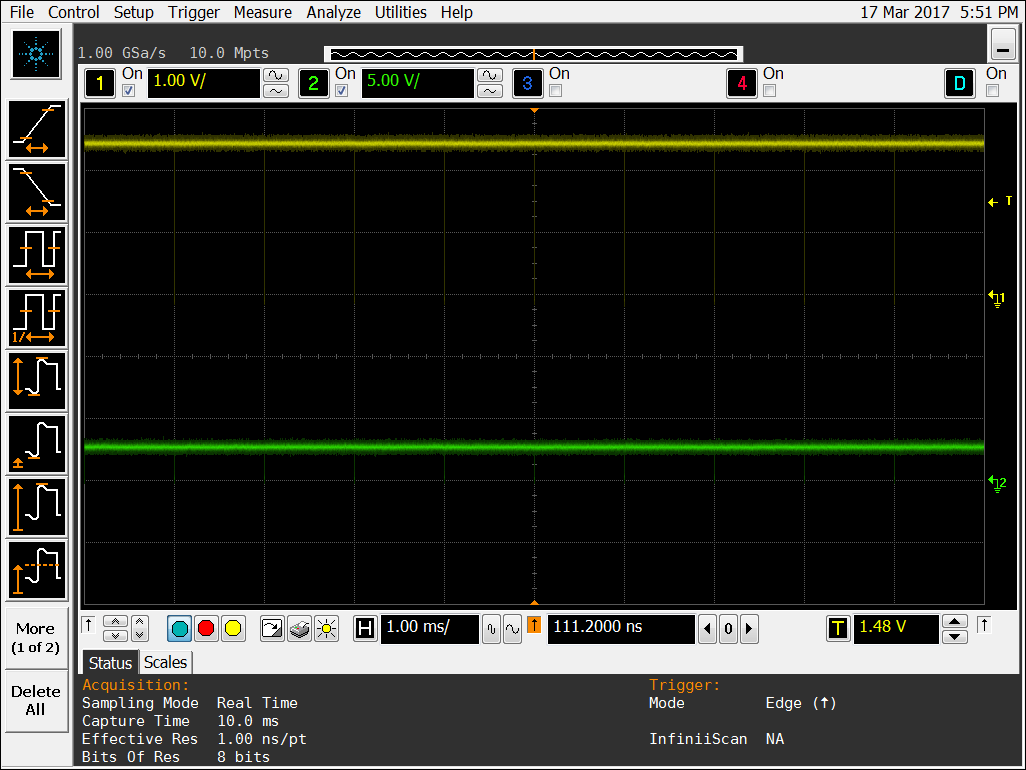
\includegraphics[width=13cm]{1khz_mb_offset_500_ns}
		\caption{Image showing a 1kHz signal produced using the internal clock of the rhino}
		\label{fig:1kHz_in_500_offset}
	\end{figure}
	
Figure \ref{fig:1kHz_in_500_offset} shows the output of the main bang and the digitisation signals measured from the Rhino board. A time division of 1.0 ms was used to display the output. Observing the yellow signal, it can seen that a 1kHz signal was indeed being produced by the Rhino board.

	\begin{figure}[t]
		\centering
		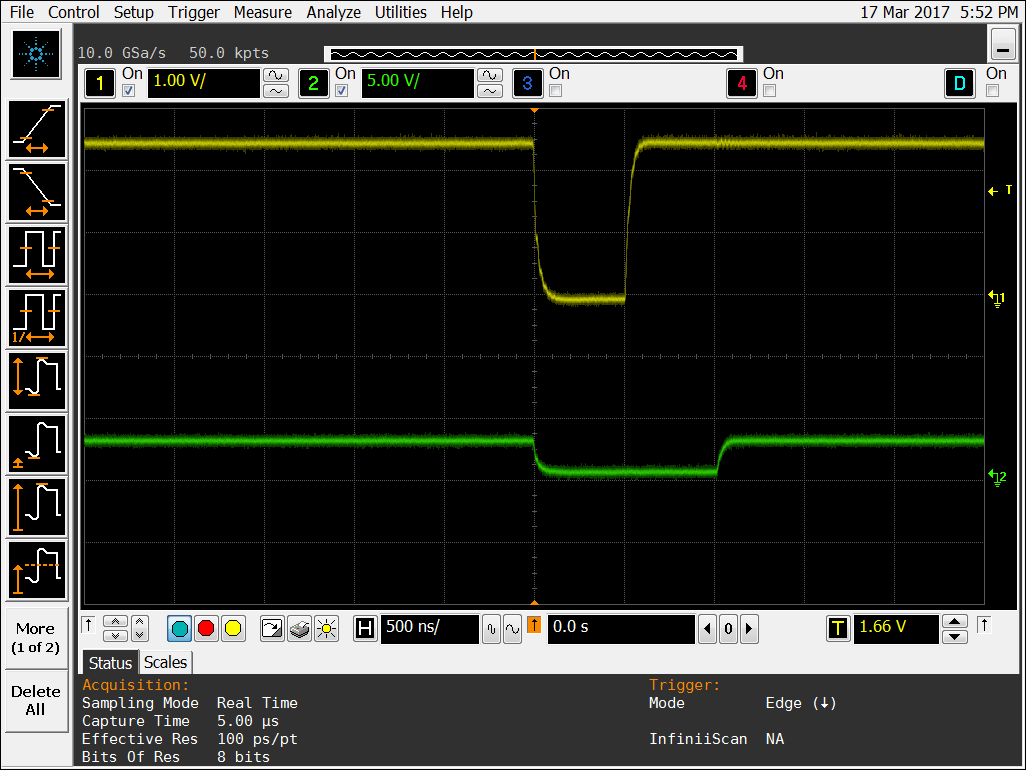
\includegraphics[width=13cm]{1khz_mb_offset_500_ns_length_of_offset}
		\caption{Zoomed in image of Figure \ref{fig:1kHz_in_500_offset}}
		\label{fig:1kHz_in_500_offset_zoom}
	\end{figure}
		
	
Figure \ref{fig:1kHz_in_500_offset_zoom} shows a zoomed in image of Figure \ref{fig:1kHz_in_500_offset}. The yellow signal depicts the main bang signal and the green signal depicts the digitization signal. The yellow signal goes high after 500ns and the green signal triggers 500ns after the yellow signal. These results are as desired. 

To change the main bang offset and the digitization offset to \hypertarget{1000ns_offset}{1000ns} without changing the other parameters, the following command was used:


	%display the echo command used to produce a signal with 1000ns offset
		\fbox{\begin{minipage}{30em}
			echo -e -n "\textbackslash x64\textbackslash x00\textbackslash x64\textbackslash x00\textbackslash x01\textbackslash x00\textbackslash x14\textbackslash x05\textbackslash x01\textbackslash x00\textbackslash x3b\textbackslash x86" $>$ /proc/$<$PID$>$/hw/ioreg/reg\textunderscore pulses
		\end{minipage}}
	
	%image showing that the main bang and digitization offset is indeed 1000ns
	\begin{figure}[t]
		\centering
		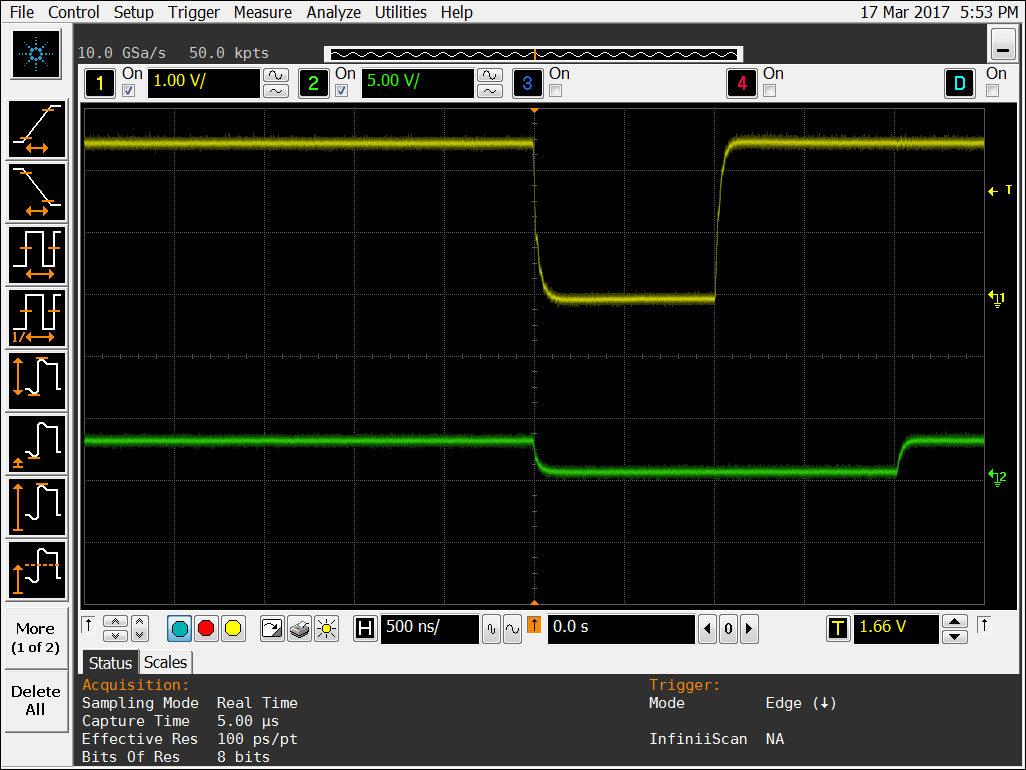
\includegraphics[width=13cm, height=8cm]{1khz_mb_offset_1000_ns_length_of_offset}
		\caption{Image of the main bang signal and digitization with 1000ns offsets}
		\label{fig:1kHz_in_1000_offset}
	\end{figure}
	

%explaining what is seen in the 1000ns image
Figure \ref{fig:1kHz_in_1000_offset} shows am image of the main bang and digitization signals with 1000ns offsets. With a 500ns time division on the horizontal axis, it can be seen that it took two time divisions for the main bang signal(yellow signal seen at the top of figure \ref{fig:1kHz_in_1000_offset}) to go high. This equates to 1000ns, which is the desired result. Similarly for the digitization signal, we see that it also took 2 time divisions to trigger, thus meeting our desired result. 

To show that the main bang offset and digitization offset can be set to different values, the main bang offset was set to 1650 ns and the digitization offset was set to 2950ns. The following command was used to set these values:

	%display the echo command used to produce a signal mb offset of 1650 ns 
	%and digitization offset of 2950ns
		\fbox{\begin{minipage}{30em}
			echo -e -n "\textbackslash xa5\textbackslash x00\textbackslash x27\textbackslash x01\textbackslash x01\textbackslash x00\textbackslash x14\textbackslash x05\textbackslash x01\textbackslash x00\textbackslash x3b\textbackslash x86" $>$ /proc/$<$PID$>$/hw/ioreg/reg\textunderscore pulses
		\end{minipage}}
		

	\begin{figure}[t]
		%\centering
   		\begin{subfigure}[t]{13.5cm}
   			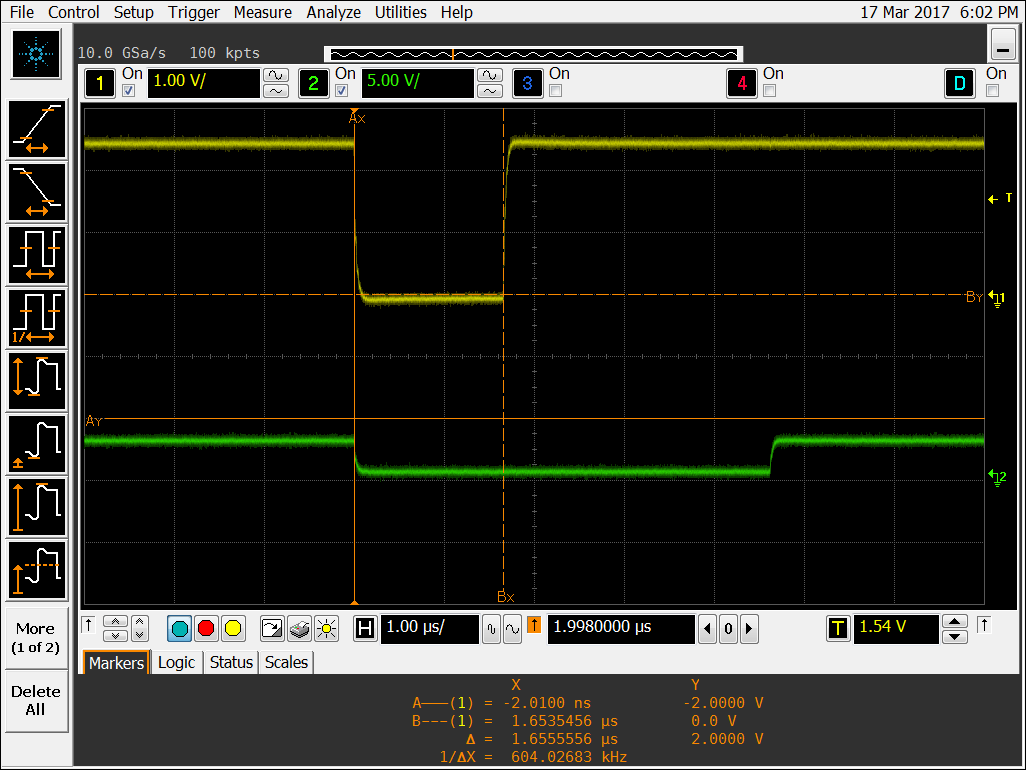
\includegraphics[width=13cm,height=8.5cm]{1khz_mb_1650ns_mb_offset}
   			\caption{}
   			\label{fig:var_offsets_1650} 
		\end{subfigure}

		\begin{subfigure}[t]{13.5cm}
   			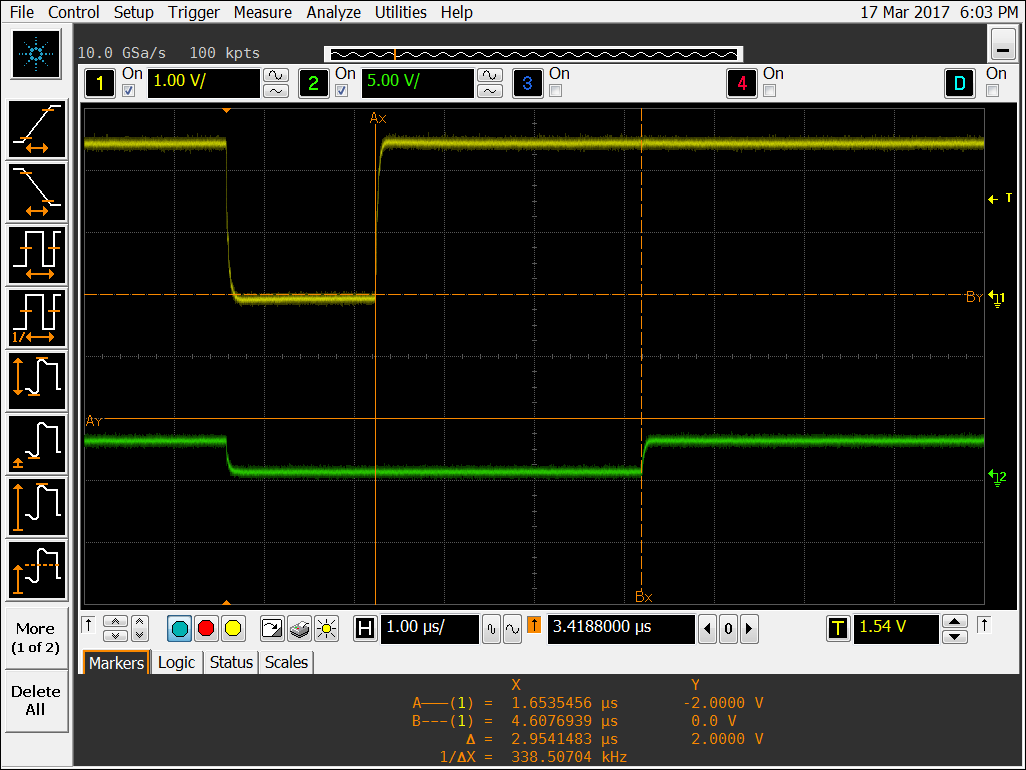
\includegraphics[width=13cm,height=8.5cm]{1khz_mb_2950ns_d_offset}
   			\caption{}
   		\label{fig:var_offsets_2950}
		\end{subfigure}

	\caption{(a) Main bang and digitization signal with the measurement of the main offset shown in the markers box toward the bottom of the image. (b) Same as figure \ref{fig:var_offsets_1650} but with the measurement of the digitization offset shown in the  markers box.}
	\label{fig:variable_offsets}
	\end{figure}

\clearpage
	
Figure \ref{fig:variable_offsets} shows the plots of the main bang signal and the digitization signal together with the measurements. Making use of cursors on the oscillscope, which allow you to measure a value on the horizontal and vertical axis, the offsets were measured. In the markers tab seen in figure \ref{fig:var_offsets_1650}, there is a delta value. From this plot, we see that \( \Delta = 1.6555556 \mu \). Observing the delta seen in figure \ref{fig:var_offsets_2950}, we see that \( \Delta = 2.9541483 \mu \). 


A main bang offset of 1650ns is equivalent to \( 1.65 \mu \). The value of delta seen in figure \ref{fig:var_offsets_1650} is thus approximately equal to the value that was set using the echo command. For the digitization offset, we set a value of 2950ns (\( 2.95 \mu \)). The delta value seen in figure \ref{fig:var_offsets_2950} is also approximately equal to the value that was set. This proves that the main bang and the digitization offsets can be set to two different values. 


	%image showing the 2kHz signal using the internal clock
	%\begin{flushleft}
	\begin{figure}[t]
		\centering
		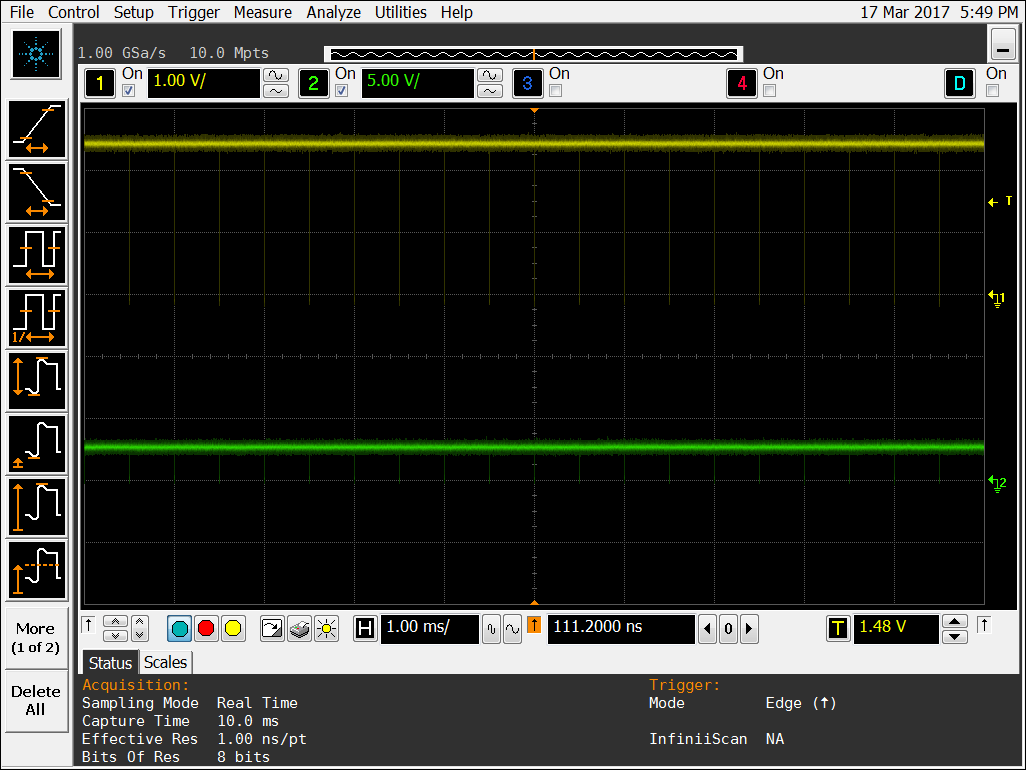
\includegraphics[width=13cm, height=8cm]{2khz_mb_offset_500_ns}
		\caption{Image showing a 2kHz signal produced using the internal clock of the Rhino board}
		\label{fig:2kHz_sig_int}
	\end{figure}
	%\end{flushleft}	
	
	%image showing the 3kHz signal using the internal clock
	%\begin{flushleft}
	\begin{figure}[t]
		\centering
		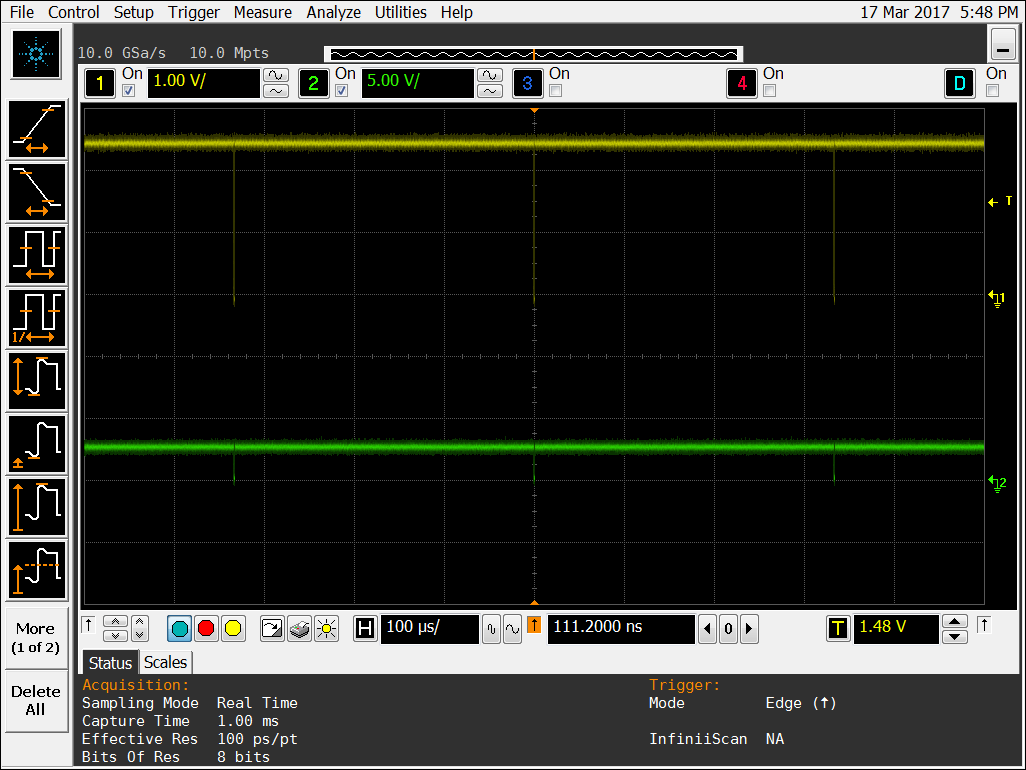
\includegraphics[width=13cm, height=8cm]{3khz_mb_offset_500_ns}
		\caption{Image showing a 3kHz signal produced using the internal clock of the Rhino board}
		\label{fig:3kHz_sig_int}
	\end{figure}
	%\end{flushleft}
	
	%image showing the 4kHz signal using the internal clock
	%\begin{flushleft}
	\begin{figure}[t]
		\centering
		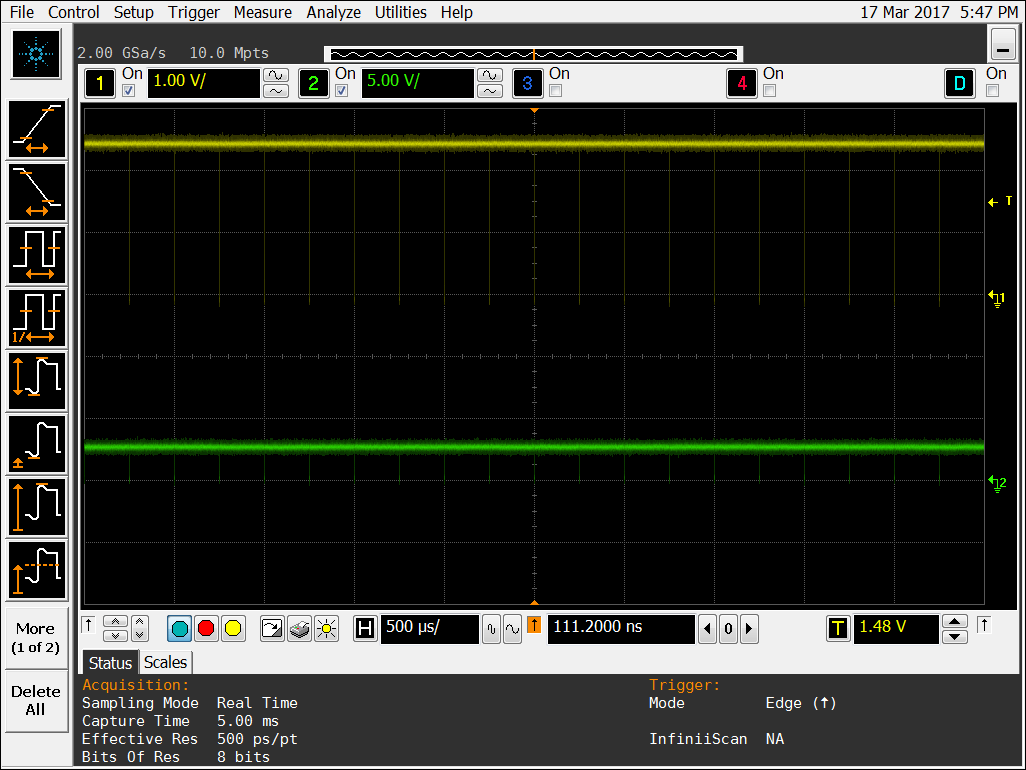
\includegraphics[width=13cm, height=8cm]{4khz_mb_offset_500_ns}
		\caption{Image showing a 4kHz signal produced using the internal clock of the Rhino board}
		\label{fig:4kHz_sig_int}
	\end{figure}
	%\end{flushleft}		


Figures \ref{fig:2kHz_sig_int}, \ref{fig:3kHz_sig_int} and \ref{fig:4kHz_sig_int} show images of the output produced when a signal with either a 2kHz, 3kHz or 4kHz frequency is set using the echo command. Each of the plots was set using a 500ns offset for the main bang and digitization offsets, using a band frequency of 1300 Mhz, operating at L-band. The only that changes when switching between frequency is the PRI that is set. 


To produce a 2kHz signal, we would need a PRI of 49899 (calculated using the equation for PRI found in section \ref{syn_control_setup}). The following command was used to set the parameters for the 2kHz signal:
	
	%echo command used to set the 2kHz signal
		\fbox{\begin{minipage}{30em}
			echo -e -n "\textbackslash x32\textbackslash x00\textbackslash x32\textbackslash x00\textbackslash x00\textbackslash x00\textbackslash x14\textbackslash x05\textbackslash x01\textbackslash x00\textbackslash xeb\textbackslash xc2" $>$ /proc/$<$PID$>$/hw/ioreg/reg\textunderscore pulses
		\end{minipage}}
		
To produce the 3kHz and 4kHz signals, the same command as above was used, the only difference being that a new PRI value was calculated and this new value plugged into the appropriate position in the command.

Observing figure \ref{fig:2kHz_sig_int}, we see that a 2kHz signal was being produced. A 1.00ms time division was being used and in 1 time division, the signal goes high twice. This equates to the signal going high every 2ms which is equivalent to 2kHz. 


Observing figure \ref{fig:3kHz_sig_int}, which has a time division of \( 100\mu s\), we see that a 3kHz is being produced. The main bang signal (yellow signal) goes high at about 3.3 time divisions. When you multiply the number of time divisions with the value of 1 time division, we get \(330\mu s\). This is equivalent to 3kHz, which is exactly what we wanted. From figure \ref{fig:4kHz_sig_int} we can see that a 4kHz signal is being produced. A time division of \(500\mu s\) is being used. Thus 1 time division is equal to 2kHz. In this picture, we see that the yellow signal went high twice for every time division. Thus, we have twice the frequency observed in a single time division. i.e. a 4khz signal is being produced.


\subsection{Using an External 100MHz Clock Signal}

Initial testing was done by making use of the internal 100MHz clock of the rhino board as mentioned in the previous section. Since the final set-up would be run using an external 100MHz clock, tests were conducted to ensure the updated synchronization controller would be able to operate correctly using an external clock.

%dont have plot of 1khz clock being produced by the external clock, but mentioned that it was observed that it looked exatcly the same as the one made
%using the internal clock.
%Add a plot of the 500ns offsets, 100ns offset and the variable offset using the internal clock. Then mention that the same plot were produced for the other signals.
The same commands used during the internal clock tests were used for the internal clock tests. The command used to setup up a signal that triggers every 1 ms (1Khz), has a main bang and digitisation offset of 500ns, a band frequency of 1300 MHz and operating at L-band is shown below. 

%display an example of the echo command inside a box
	\fbox{\begin{minipage}{30em}
			echo -e -n "\textbackslash x32\textbackslash x00\textbackslash x32\textbackslash x00\textbackslash x01\textbackslash x00\textbackslash x14\textbackslash x05\textbackslash x01\textbackslash x00\textbackslash x3b\textbackslash x86" $>$ /proc/$<$PID$>$/hw/ioreg/reg\textunderscore pulses
	\end{minipage}}

	%image showing the output of 1khz clock
	\begin{figure}[t]
		\centering
		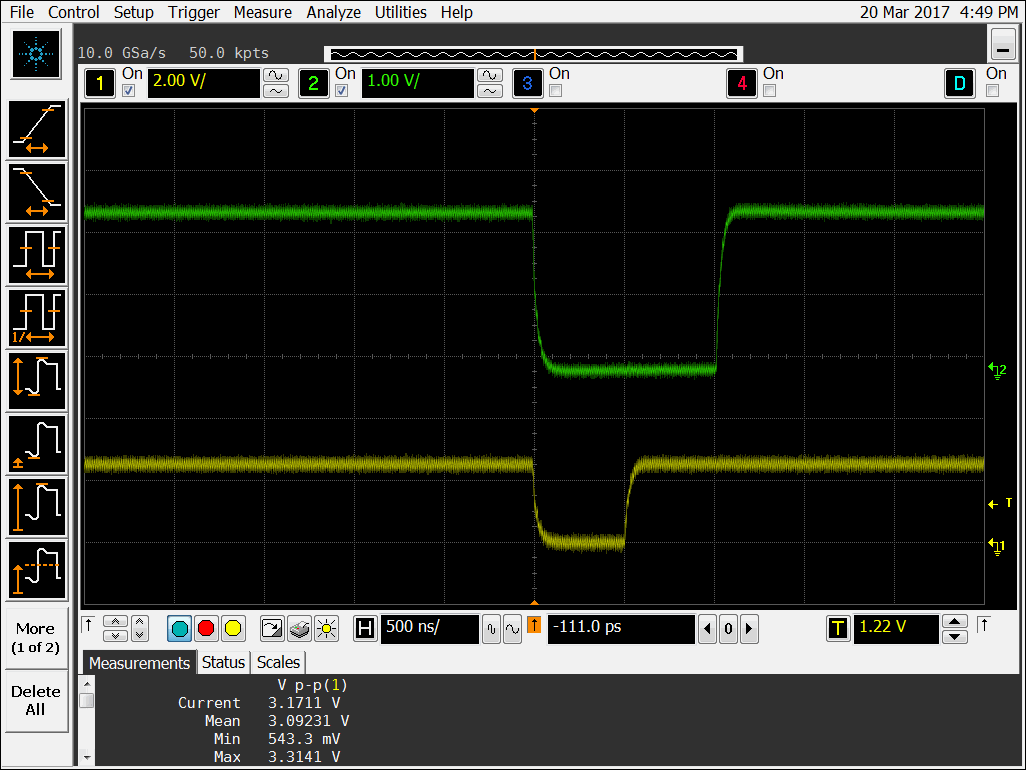
\includegraphics[width=13cm]{1khz_ext_mb_500ns}
		\caption{Image showing a 1khz main bang signal(yellow) and the associated digitization signal, both with an offset of 500ns}
		\label{fig:1khz_sig_ext}
	\end{figure}

Figure \ref{fig:1khz_sig_ext} shows the output produced by using the above command. A 500ns time division was used to display the output. The yellow signal (bottom signal) represents the main bang signal and the green signal represents the digitization signal. As can be seen in the image, it took a single time division for the main bang signal to trigger high. The digitization signal took a further 500ns to do the same. We set the main bang and digitization offsets to 500ns and figure \ref{fig:1khz_sig_ext} proves that these values are correctly set up. The output seen in figure \ref{fig:1khz_sig_ext} is also in agreement with the output seen in figure \ref{fig:1kHz_in_500_offset_zoom}. 

	%figure showing the output when a 1000ns offset was set
	\begin{figure}[t]
		\centering
		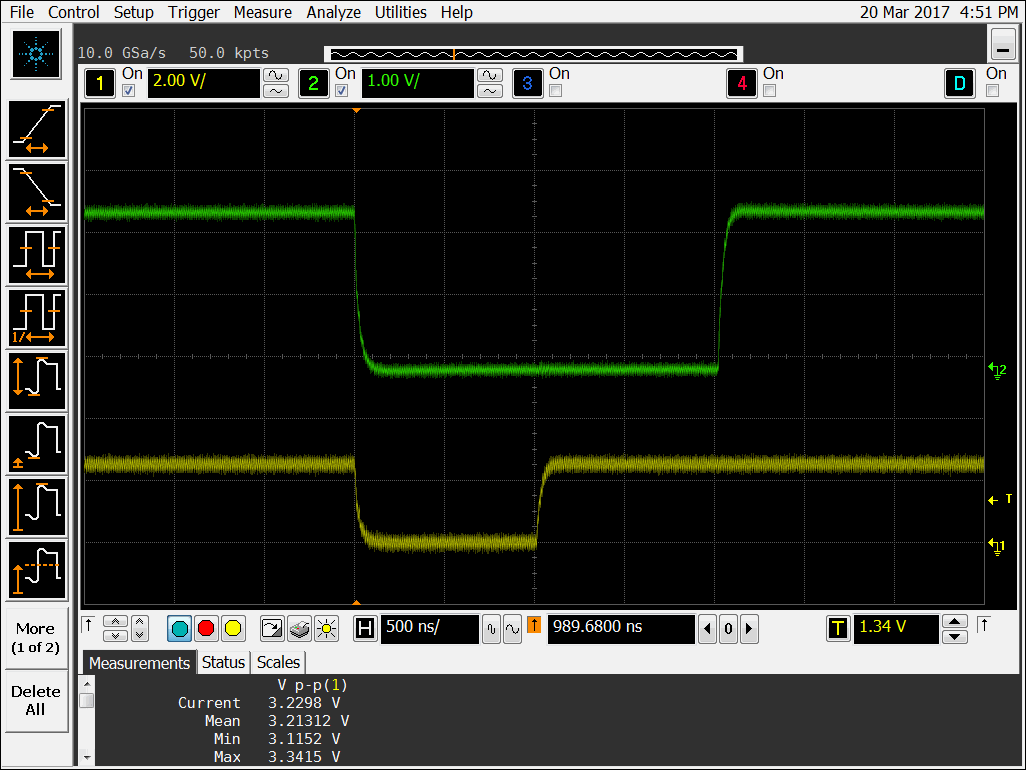
\includegraphics[width=13cm]{1khz_ext_mb_d_offset_1000ns}
		\caption{Image showing a 1khz main bang signal(yellow) and the associated digitization signal(green), both with an offset of 1000ns}
		\label{fig:1khz_ext_sig_1000ns_offset}
	\end{figure}

To change the main bang offset and the digitization offset, the same command used in previous section was used. The command can be found \hyperlink{1000ns_offset}{here}. The output produced after making the change can be seen in figure \ref{fig:1khz_ext_sig_1000ns_offset}. A time division of 500ns was used to display the image. Observing the yellow (main bang) signal, we see that it took 2 time divisions for the signal to trigger high. This means that it took 1000ns in total. A similar observation was made about the green (Digitization) signal.

Tests were then done to see if the 2kHz, 3kHz and 4kHz signals could be produced using the external clock. The commands used to set the rhino to produce to appropriate commands are shown below.

The following command was used to set the rhino up to produce a 2kHz main bang signal:

	%command used to produce a 2kHz signal
	\fbox{\begin{minipage}{30em}
		echo -e -n "\textbackslash x32\textbackslash x00\textbackslash x32\textbackslash x00\textbackslash x00\textbackslash x00\textbackslash x14\textbackslash x05\textbackslash x01\textbackslash x00\textbackslash xeb\textbackslash xc2" $>$ /proc/$<$PID$>$/hw/ioreg/reg\textunderscore pulses
	\end{minipage}}

The produce the 3kHz signal, this command was used:

	%command used to produce a 3kHz signal
	\fbox{\begin{minipage}{30em}
		echo -e -n "\textbackslash x32\textbackslash x00\textbackslash x32\textbackslash x00\textbackslash x00\textbackslash x00\textbackslash x14\textbackslash x05\textbackslash x01\textbackslash x00\textbackslash xd0\textbackslash x81" $>$ /proc/$<$PID$>$/hw/ioreg/reg\textunderscore pulses
	\end{minipage}}

And to produce the 4kHz signal, this command was used:

	%command used to produce a 4kHz signal
	\fbox{\begin{minipage}{30em}
		echo -e -n "\textbackslash x32\textbackslash x00\textbackslash x32\textbackslash x00\textbackslash x00\textbackslash x00\textbackslash x14\textbackslash x05\textbackslash x01\textbackslash x00\textbackslash x43\textbackslash x61" $>$ /proc/$<$PID$>$/hw/ioreg/reg\textunderscore pulses
	\end{minipage}}

Similar to what was done for the internal clock tests, each of the signals was set using a 500ns offset for the main bang and digitization offsets, using a band frequency of 1300 Mhz, operating at L-band. The only that changes when switching between frequency is the PRI that is set. The only difference being that the value that was specified for the signal.

%when explaing the output, display an image and expain some stuff, then display another image and show some stuff and so forth

	%figure showing the output of a 2Khz signal using an external clock 
	\begin{figure}[t]
		\centering
		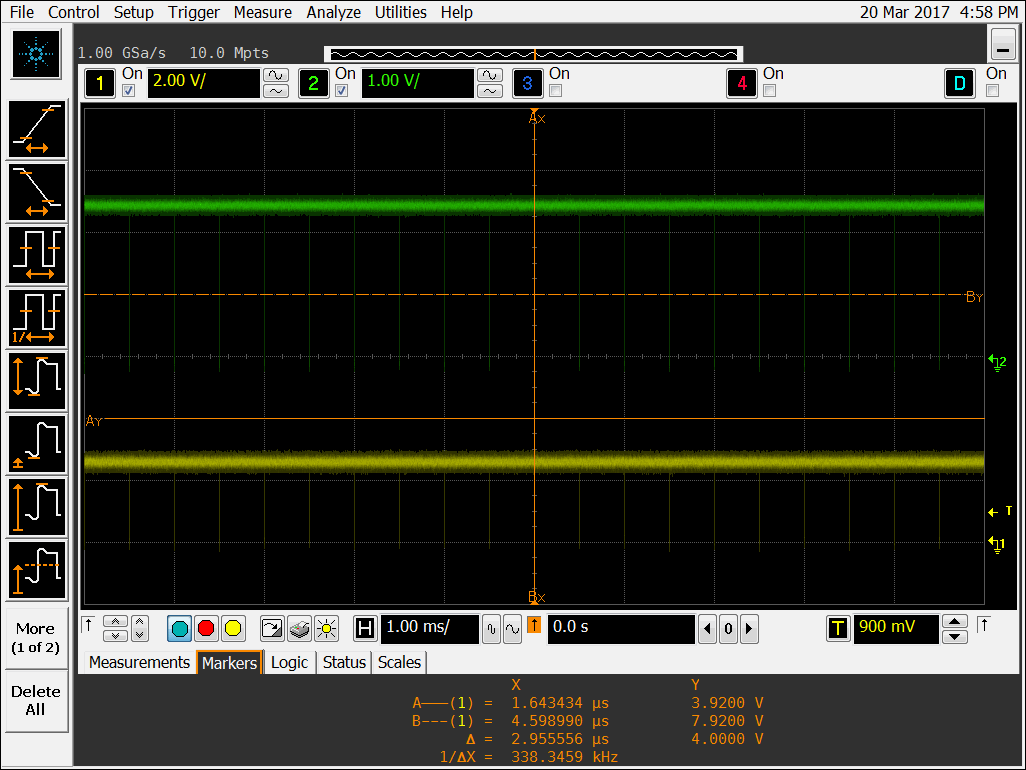
\includegraphics[width=13cm]{2khz_ext_500ns}
		\caption{Image showing a 2kHz main bang signal (green) and the digitization signal (yellow)}
		\label{fig:2khz_ext_sig}
	\end{figure}

Figure \ref{fig:2khz_ext_sig} shows an image of the output produced when a 2kHz signal was set. A 1ms time division was used to display the output. Observing the green signal, which represents the main bang signal, we see that the signal goes high twice in a single time division. This means that we have twice the frequency represented by a single time division. In this, it means that the a 2kHz signal is being produced by the main bang signal output of the rhino board. This is what was expected.

	%figure showing the output of a 3Khz and 4kHz signals using an external clock 
	\begin{figure}[t]
		%\centering
		\begin{subfigure}{13.5cm}
			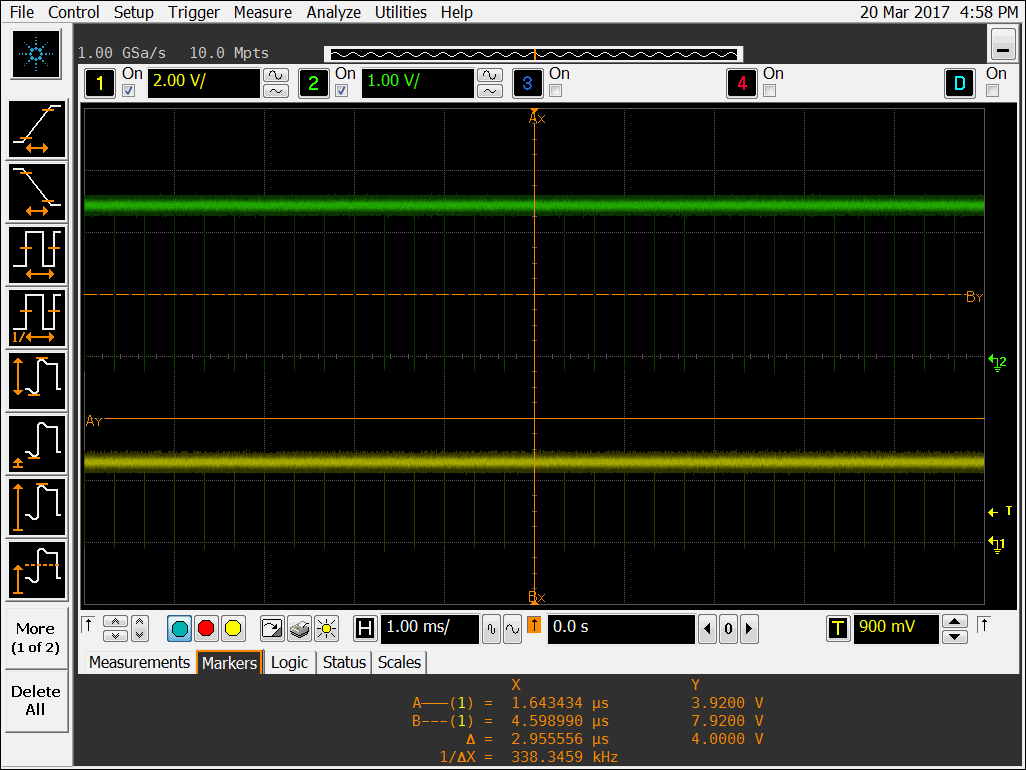
\includegraphics[width=13cm,height=8.5cm]{3khz_ext_500ns}
			\caption{}
			\label{fig:3khz_ext_sig} 
		\end{subfigure}
		
		\begin{subfigure}{13.5cm}
			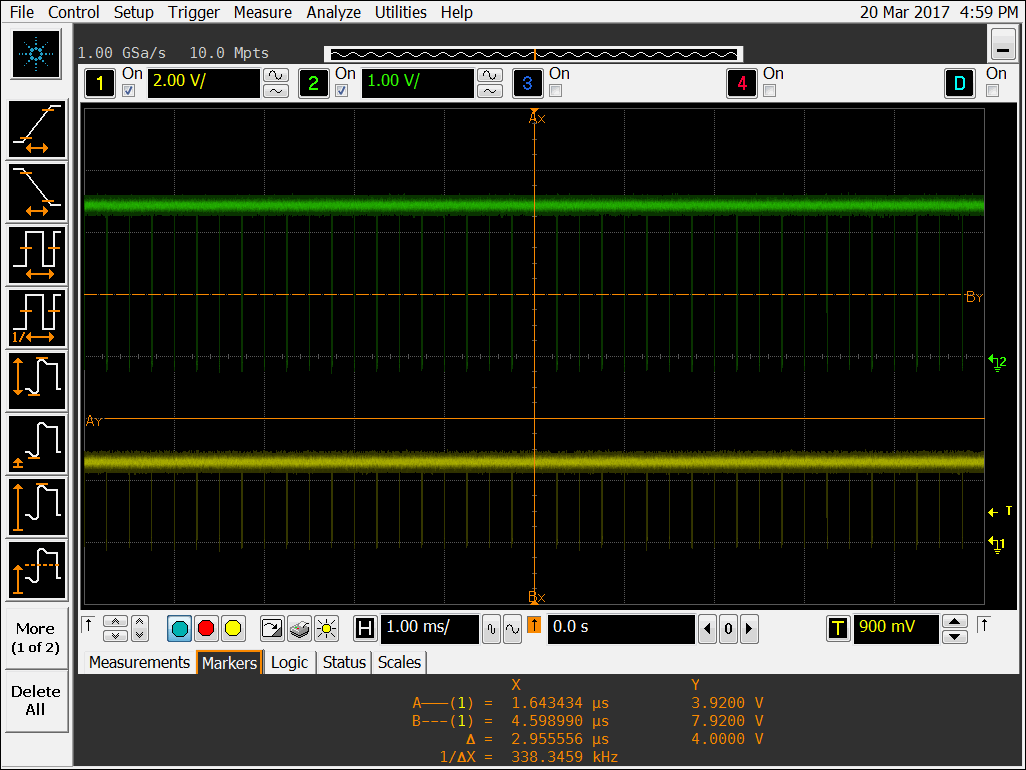
\includegraphics[width=13cm,height=8.5cm]{4khz_ext_500ns}
			\caption{}
			\label{fig:4khz_ext_sig}
		\end{subfigure}
		
		\caption{(a) Main bang and digitization signal produced when the rhino was set up to produce a main bang signal of 3kHz. (b) Same as (a) but for the case when a 4kHz signal was set up}
		\label{fig:3_4_khz_ext_sig}
	\end{figure}

Figure \ref{fig:3_4_khz_ext_sig} shows images of the output produced when a 3kHz and 4kHz signals were set up using the aforementioned commands. A 1ms time division was used to display the output. From figure \ref{fig:3khz_ext_sig}, we see that the main bang signal goes high about 3 times in a single time division. The time interval between each trigger high level is evenly spaced. This means that the frequency of the main bang signal is indeed 3kHz. Similarly, in figure \ref{fig:4khz_ext_sig}, we see that the main bang signal goes high about 4 times in a single time division. This means that the frequency of the main bang signal in the second figure is 4kHz.

\section{Conclusions}

%mention how after making the modifications to the original coce, I was able to show that various signals were able to be produced
%and that the offsets can be changed to any desired value

Modifying the PRI register size from 16 bits to 32 bits has not affected the rest of the functionality of the TCU controller. As observed in the results section, a user would be to set the main bang offset, digitization offset and other parameters to their desired values and the rhino would produce behaviour which closely approximates the set values for these parameters.

Additionally, it was proven that the rhino was capable of accepting a 32 bit value for the PRI offset and able to produce a main bang signal of some specified frequency.

\section{Recommendations}

%mention that the CLI c code and the gui need to be updated to reflect the changes that I made to my code

The CLI(Command line Interface) program and the gui for the TCU need to be updated to so that they can handle 32 bit values for the PRI offset.

\end{document}